\documentclass[a4paper,11pt,fleqn]{article}%fleqn pour aligner les equations à gauche
\usepackage{../../Styles/Exercice}


\newcommand{\chnum}{Chapitre 12}
\newcommand{\chtitle}{Modéliser une action sur un système}
\newcommand{\dtype}{Exercices}

\begin{document}
\maketitle

\begin{multicols}{2}
\section{Questions d'introduction}
\begin{enumerate}
    \item En mathématiques, on parle de "norme" d'un vecteur. Donner deux équivalents en physique.
    \item Rappeler l'origine physique du poids d'un objet sur Terre
    \item L'eau liquide des océans permet aux icebergs de flotter. Déterminer la nature de l'action mécanique mise en jeu.
    \item Un aigle a une masse de \SI{5}{kg}.
    \begin{itemize**}
        \item Représenter le vecteur poids sans souci d'échelle.
        \item Donner ses caractéristiques
    \end{itemize**}
    \item Une voiture est garée dans une rue en pente de Montréal. Représenter la résultante des forces de contact exercées par la route sur la voiture.
    \item Calculer la masse d'un globule rouge dont le poids sur Terre est \SI{0,40}{\pico\newton}. rappel : $\SI{1}{\pico\newton} = \SI{1E-12}{N}$.
\end{enumerate}

\section{Modéliser une force par un vecteur}
Léa d'est rendue à la bibliothèque pour étudier l'interaction gravitationnelle. A coté des \oe uvres de Newton, elle trouve un vieil ouvrage écrit par Galilée. Curieuse, elle l'emprunte et le pose sur la table.
\begin{enumerate}
    \item Donner les caractéristiques des forces d'exerçant sur l'ouvrage de Léa.
    \item Représenter vectoriellement ces forces en prenant pour échelle de représentation \SI{1}{cm} = \SI{2}{N}.
\end{enumerate}
\textbf{Données :}
\begin{itemize}
    \item \textbf{Masse de l'ouvrage de Léa :} $m=\SI{600}{g}$
    \item \textbf{intensité de pesanteur :} $g=\SI{9,81}{\newton\per\kilo\gram}$
\end{itemize}

\section{Exemples de forces caractéristiques}
La Terre et la Lune sont en interaction gravitationnelle.
\begin{itemize}
    \item Donner la direction, le sens et l'expression littérale de la force qu'exerce la Terre sur la Lune.
\end{itemize}

\section{La tour de pise}
\begin{minipage}{.5\linewidth}
\begin{enumerate}
    \item Déterminer les forces s'appliquant sur la tour de Pise.
    \item Représenter ces forces sur un schéma sans soucis d'échelle.
    \item Hormis les normes, quelles sont les caractéristiques des vecteurs forces mis en jeu ?
\end{enumerate}
\end{minipage}
\begin{minipage}{.3\linewidth}
    \centering
    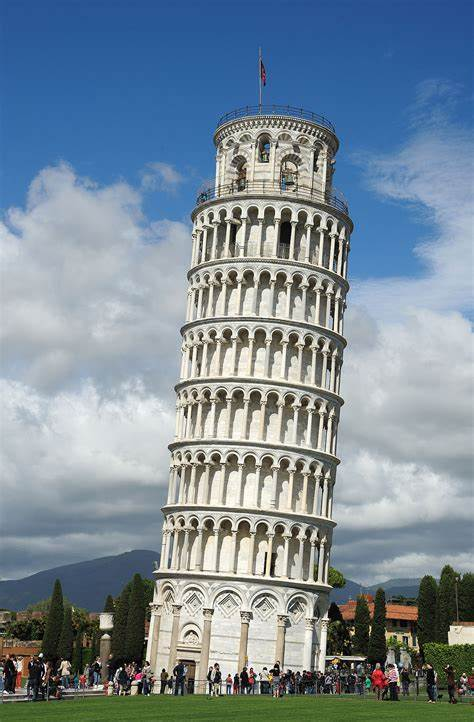
\includegraphics[width=\linewidth]{Ressources/2GT_C7_Exercices_Fig1.jpg}
\end{minipage}
\section{Formule de la force d'interaction gravitationnelle}
\begin{enumerate}
    \item Rappeler la formule donnant la valeur de la force d'interaction gravitationnelle entre deux objets $A$ et $B$ de masses $m_A$ et $m_B$ distants de $d$. On précisera les unités.
    \item Calculer la valeur de cette force dans le cas du Soleil et de Jupiter.
\end{enumerate}
\textbf{Données :}
\begin{itemize**}
    \item $m_{Jupiter} = \SI{1,90E27}{kg}$
    \item $m_{Soleil} = \SI{1,99E30}{kg}$
    \item $d = \SI{7,79E8}{km}$
    \item $G = \SI{6,67E-11}{\newton\meter\squared\per\kilo\gram\squared}$
\end{itemize**}

\section{Le principe des actions réciproques}
Jean est à la piscine. Il participe à une compétition de 100 mètres nage libre. Au bout de 50 mètres, il fait demi-tour en poussant sur le mur avec ses pieds.
\begin{itemize}
    \item A l'aide du principe des actions réciproques, justifier l'interêt pour Jean d'utiliser le mur pour faire un demi-tour.
\end{itemize}
\end{multicols}
\end{document}